\chapter{Specifikacija programske potpore}
		
	\section{Funkcionalni zahtjevi}
			
			\noindent \textbf{Dionici:}
			
			\begin{packed_enum}
				
				\item Korisnik
				    \begin{packed_item}
				    \item Pacijent
				    \item Liječnik
				    \item Medicinski tehničar/sestra
				    \end{packed_item}
				\item Administrator
				\item Naručitelj
				\item Razvojni tim
			\end{packed_enum}
			
			\noindent \textbf{Aktori i njihovi funkcionalni zahtjevi:}
			
			
			\begin{packed_enum}
				
				\item  \underbar{Neregistrirani/neprijavljeni korisnik (inicijator) može:}
				
				\begin{packed_enum}
					
					\item pregledati naslovnu stranicu za neprijavljene korisnike
					\item se registrirati u sustav kao pacijent, stvoriti novi korisnicki račun za koji su mu potrebni e-mail adresa, lozinka, ime, prezime, spol, broj mobitela i odabrani liječnik
					
				\end{packed_enum}
				
				\item  \underbar{Pacijent (inicijator) može:}
				
				\begin{packed_enum}
					
					\item pregledati naslovnu stranicu za pacijente, svoj kalendar sa zakazanim pregledima i prozor za poruke o pomaknutim terminima
					\item potvrditi ili odbiti pomaknute termine
					\item odabrati pregled kod liječnika ili specifičnu vrstu usluge kod medicinskog tehničara/sestre, te zakazati termin
					\item zakazani termin otkazati
					\item dobiti podsjetnik na pregled, ili obavijest o pomaknutom pregledu na svoj e-mail ili sms
					
				\end{packed_enum}
				
				\item  \underbar{Liječnik (inicijator) može:}
				
				\begin{packed_enum}
					
					\item pregledati naslovnu stranicu za liječnike, svoj kalendar s rezerviranim terminima
					\item za rezervirane termine vidjeti tip pregleda i podatke o pacijentu
					\item definirati raspoloživost termina
					\item definirati vlastita pravila o rezervaciji termina i proizvoljno iz mijenjati
					\item pomaknuti rezervirani termin
					\item unositi potvrdu dolaska pacijenta na rezervirani termin
					
				\end{packed_enum}
				
				\item  \underbar{Medicinski tehničar/sestra (inicijator) može:}
				
				\begin{packed_enum}
					
					\item pregledati naslovnu stranicu za medicinskog tehničara, svoj kalendar sa rezerviranim terminima
					\item za rezervirane termine vidjeti vrstu specifične usluge
					\item definirati slobodne termine za specifične vrste usluga
					\item pomaknuti rezervirani termin
					\item unositi potvrdu dolaska pacijenta na rezervirani termin
					
				\end{packed_enum}
				
				\item  \underbar{Administrator (inicijator) može:}
				
				\begin{packed_enum}
					
					\item kreirati specijalizirane tipove korisnika (liječnik i medicinski tehničar/sestra)
					\item kreirati medicinske timove u kojima grupa liječnike i medicinske tehničare/sestre
					
				\end{packed_enum}
				
				\item  \underbar{Baza podataka (sudionik):}
				
				\begin{packed_enum}
					
					\item pohranjuje sve podatke o korisnicima i njihovim ovlastima
					\item pohranjuje sve podatke o zakazanim i slobodnim terminima
					
				\end{packed_enum}
				
				\item  \underbar{Sustav (sudionik):}
				
				\begin{packed_enum}
					
					\item generira izvješća o učinkovitosti rezervacije i šalje ih u informacijski sustav HZZO-a

				\end{packed_enum}
				
				
			\end{packed_enum}
			
			\eject 
			
			
				
			\subsection{Obrasci uporabe}
				
				\subsubsection{Opis obrazaca uporabe}
				
				    \noindent \underbar{\textbf{UC1 - Registracija}}
					\begin{packed_item}
	
						\item \textbf{Glavni sudionik: }Korisnik
						\item  \textbf{Cilj:} Registrirati korisnika u sustav
						\item  \textbf{Sudionici:} Baza podataka
						\item  \textbf{Preduvjet:} -
						\item  \textbf{Opis osnovnog tijeka:}
						
						\item[] \begin{packed_enum}
	
							\item Korisnik odabire opciju za registraciju
							\item Korisnik unosi potrebne podatke
							\item Pristiskom na dugme potvrđuje registraciju
							\item Po uspješnoj registraciji korisnik zaprima potvrdu na registriranu adresu e-pošte
							\item Pristup korisničkim funkcijama sukladno njegovom korisničkom tipu
						\end{packed_enum}
						
						\item  \textbf{Opis mogućih odstupanja:}
						
						\item[] \begin{packed_item}
	
							\item[2.a] Odabir već zauzetog e-maila, unos podataka u nedozvoljenom formatu ili pružanje neispravnoga e-maila 
							\item[] \begin{packed_enum}
								
								\item Sustav obavještava korisnika o neuspjelom upisu i vraća ga na stranicu za registraciju
								\item Korisnik mijenja potrebne podatke te završava unos ili odustaje od registracije
								
							\end{packed_enum}
						\end{packed_item}
					\end{packed_item}
				
				
					\noindent \underbar{\textbf{UC2 - Prijava u sustav}}
					\begin{packed_item}
	
						\item \textbf{Glavni sudionik: }Korisnik
						\item  \textbf{Cilj:} Prijaviti korisnika u sustav
						\item  \textbf{Sudionici:} Baza podataka
						\item  \textbf{Preduvjet:} Registracija
						\item  \textbf{Opis osnovnog tijeka:}
						
						\item[] \begin{packed_enum}
	                        
	                        \item Korisnik odabire opciju za prijavu
							\item Unos korisničkog imena i lozinke
							\item Pristiskom na dugme potvrđuje prijavu
							\item Pristup korisničkim funkcijama sukladno njegovom korisničkom tipu
						\end{packed_enum}
						
						\item  \textbf{Opis mogućih odstupanja:}
						
						\item[] \begin{packed_item}
	
							\item[2.a] Neispravno korisničko ime/lozinka
							\item[] \begin{packed_enum}
								
								\item Sustav obavještava korisnika o neuspjelom upisu i vraća ga na stranicu za prijavu
								\item Korisnik mijenja potrebne podatke te završava unos ili odustaje od prijave
							\end{packed_enum}
						\end{packed_item}
					\end{packed_item}
					
					\noindent \underbar{\textbf{UC3 - Pregled zakazanih termina}}
					\begin{packed_item}
	
						\item \textbf{Glavni sudionik: } Pacijent
						\item  \textbf{Cilj:} Omogućiti pacijentu uvid u zakazane termine
						\item  \textbf{Sudionici:} Baza podataka
						\item  \textbf{Preduvjet:} Korisnik prijavljen kao pacijent
						\item  \textbf{Opis osnovnog tijeka:}
						
						\item[] \begin{packed_enum}
	
							\item Korisniku se prikaže naslovna stranica za pacijente
							\item Korisnik na vlastitom kalendaru ima uvid u svoje termine
						\end{packed_enum}
						
					\end{packed_item}
					
					\noindent \underbar{\textbf{UC4 - Zakazivanje termina kod liječnika}}
					\begin{packed_item}
	
						\item \textbf{Glavni sudionik: }Pacijent
						\item  \textbf{Cilj:} Omogućiti pacijentu odabir termina pregleda kod liječnika
						\item  \textbf{Sudionici:} Baza podataka
						\item  \textbf{Preduvjet:} Prijavljen korisnik kao pacijent
						\item  \textbf{Opis osnovnog tijeka:}
						
						\item[] \begin{packed_enum}
	
							\item Korisniku se prikaže naslovna stranica za pacijente
							\item Korisnik odabire opciju zakazivanja pregleda kod liječnika 
							\item Na prikazanom kalendaru odabire željeni slobodni termin
							\item Dodatno naznačuje tip pregleda
							\item Pristiskom na dugme potvrđuje odabrani termin
							\item Korisnik dobiva potvrdu o uspješno odabranom terminu na preferirani kanal komunikacije
							\item Korisnikov kalendar se osvježava novim podacima
						\end{packed_enum}
						
						\item  \textbf{Opis mogućih odstupanja:}
						
						\item[] \begin{packed_item}
	
							\item[2.a] Korisnik je previše puta rezervirao termine
							\item[] \begin{packed_enum}
								
								\item Sustav onemogućuje zakazivanje termina i korisniku šalje odgovarajuću poruku
								\item Korisnik je preusmjeren natrag na svoju naslovnu stranicu
							\end{packed_enum}
							
							\item[2.b] Korisnik se previše puta nije pojavio na zakazanom terminu
							\item[] \begin{packed_enum}
								
								\item Sustav onemogućuje zakazivanje termina i korisniku šalje odgovarajuću poruku
								\item Korisnik je preusmjeren natrag na svoju naslovnu stranicu
							\end{packed_enum}
						\end{packed_item}
					\end{packed_item}
					
					\noindent \underbar{\textbf{UC5 - Zakazivanje termina kod medicinskog tehničara}}
					\begin{packed_item}
	
						\item \textbf{Glavni sudionik: }Pacijent
						\item  \textbf{Cilj:} Omogućiti pacijentu odabir termina usluge kod medicinskog tehničara
						\item  \textbf{Sudionici:} Baza podataka
						\item  \textbf{Preduvjet:} Prijavljen korisnik kao pacijent
						\item  \textbf{Opis osnovnog tijeka:}
						
						\item[] \begin{packed_enum}
	
							\item Korisniku se prikaže naslovna stranica za pacijente
							\item Korisnik odabire zakazivanje pregleda kod medicinskog tehničara
							\item Korisnik odabire vrstu usluge unutar predefiniranih termina
							\item Pristiskom na dugme potvrđuje odabranu uslugu
							\item Sustav korisniku dodjeljuje prvi slobodni termin
							\item Korisnik dobiva potvrdu o uspješno odabranom terminu na preferirani kanal komunikacije
							\item Korisnikov kalendar se osvježava novim podacima
						\end{packed_enum}
						
						\item  \textbf{Opis mogućih odstupanja:}
						
						\item[] \begin{packed_item}
	
							\item[2.a] Korisnik je previše puta rezervirao termine
							\item[] \begin{packed_enum}
								
								\item Sustav onemogućuje zakazivanje termina i korisniku šalje odgovarajuću poruku
								\item Korisnik je preusmjeren natrag na svoju naslovnu stranicu
							\end{packed_enum}
							
							\item[2.b] Korisnik se previše puta nije pojavio na zakazanom terminu
							\item[] \begin{packed_enum}
								
								\item Sustav onemogućuje zakazivanje termina i korisniku šalje odgovarajuću poruku
								\item Korisnik je preusmjeren natrag na svoju naslovnu stranicu
							\end{packed_enum}
						\end{packed_item}
					\end{packed_item}
					
					
					\noindent \underbar{\textbf{UC6 - Otkazivanje termina}}
					\begin{packed_item}
	
						\item \textbf{Glavni sudionik: }Pacijent
						\item  \textbf{Cilj:} Omogućiti pacijentu otkazivanje termina
						\item  \textbf{Sudionici:} Baza podataka
						\item  \textbf{Preduvjet:} Prijavljen korisnik kao pacijent,  postoji zakazan pregled
						\item  \textbf{Opis osnovnog tijeka:}
						
						\item[] \begin{packed_enum}
	
							\item Korisniku se prikaže naslovna stranicu za pacijente
							\item Korisnik na prikazanom kalendaru odabire zakazani termin
							\item Korisnik odabire opciju za otkazivanje pregleda
							\item Pristiskom na dugme potvrđuje odabranu opciju
							\item Korisnik dobiva potvrdu o uspješno otkazanom terminu na preferirani kanal komunikacije
							\item Korisnikov kalendar se osvježava novim podacima
							
						\end{packed_enum}
						
						\item  \textbf{Opis mogućih odstupanja:}
						
						\item[] \begin{packed_item}
	
							\item[2.a] Korisnik je pokušao otkazati termin 24 sata nakon zakazivanja
							\item[] \begin{packed_enum}
								
								\item Sustav onemogućuje otkazivanje i korisniku šalje odgovarajuću poruku
								\item Korisnik je preusmjeren natrag na svoju naslovnu stranicu
								
							\end{packed_enum}
						\end{packed_item}
						
					\end{packed_item}
					
					
					
					\noindent \underbar{\textbf{UC7 - Potvrđivanje novih termina nakon pomicanja}}
					\begin{packed_item}
	
						\item \textbf{Glavni sudionik: }Pacijent
						\item  \textbf{Cilj:} Pacijentu omogućiti potvrdu ili odbijanje novog termina
						\item  \textbf{Sudionici:} Baza podataka
						\item  \textbf{Preduvjet:} Korisnik prikavljen kao pacijent, liječniki tim je pomaknuo zakazani termin
						\item  \textbf{Opis osnovnog tijeka:}
						
						\item[] \begin{packed_enum}
	                        
	                        \item Sustav korisniku šalje poruku o promjenjenom terminu
							\item Korisniku se prikaže naslovna stranicu za pacijente
							\item Korisniku se u posebnom prozoru prikaže poruka o promjeni uz opcije prihvaćanja promjene
							\item Korisnik odabire opciju za prihvačanje novog termina
							\item Pristiskom na dugme potvrđuje odabranu opciju
							\item Korisnik dobiva potvrdu o uspješno prihvačenom ili odbijenom terminu na preferirani kanal komunikacije
							\item Korisnikov kalendar se osvježava novim podacima
						\end{packed_enum}
						
					
					\end{packed_item}
					
					\noindent \underbar{\textbf{UC8 - Podsjećanje pacijenta na zakazani termin}}
					\begin{packed_item}
	
						\item \textbf{Glavni sudionik: }-
						\item  \textbf{Cilj:} Slanje podsjetnika pacijentu na termin
						\item  \textbf{Sudionici:} Baza podataka, pacijent
						\item  \textbf{Preduvjet:} Postoji zakazani termin
						\item  \textbf{Opis osnovnog tijeka:}
						
						\item[] \begin{packed_enum}
	
							\item Prikupljanje podataka o pregledu i preferiranom kanalu komunikacije
							\item Konverzija u željeni oblik
							\item Slanje podsjetnika pacijentu putem preferiranog kanala komunikacije
						\end{packed_enum}
						
						\item  \textbf{Opis mogućih odstupanja:}
						
						\item[] \begin{packed_item}
	
							\item[3.a] Sustav nije mogao poslati podsjetnik zbog greške u e-mail/sms sustavu
							\item[] \begin{packed_enum}
								
								\item Sustav šalje podsjetnik putem opcionalnog kanala komunikacije
						
							\end{packed_enum}
							
						\end{packed_item}
					\end{packed_item}
					
					\noindent \underbar{\textbf{UC9 - Pregled rezeviranih termina}}
					\begin{packed_item}
	
						\item \textbf{Glavni sudionik: } Liječnik, medicinski tehničar
						\item  \textbf{Cilj:} Omogućiti medicinskom osoblju uvid u zakazane termine s dodatnim informacijama
						\item  \textbf{Sudionici:} Baza podataka
						\item  \textbf{Preduvjet:} Korisnik prijavljen kao liječnik ili medicinski tehničar
						\item  \textbf{Opis osnovnog tijeka:}
						
						\item[] \begin{packed_enum}
	
							\item Korisniku se prikaže naslovna stranica za liječnike ili medicinske tehničare
							\item Pritiskom na željeni termin u kalenadru korisnik dobije više informacija
							
						\end{packed_enum}
					\end{packed_item}
					
					\noindent \underbar{\textbf{UC10 - Potvrđivanje dolaznosti pacijenta}}
					\begin{packed_item}
	
						\item \textbf{Glavni sudionik: } Liječnik, medicinski tehničar
						\item  \textbf{Cilj:} Omogućiti medicinskom osoblju potvrđivanje dolaznosti pacijenta
						\item  \textbf{Sudionici:} Baza podataka
						\item  \textbf{Preduvjet:} Korisnik prijavljen kao liječnik ili medicinski tehničar, završio zakazani termin
						\item  \textbf{Opis osnovnog tijeka:}
						
						\item[] \begin{packed_enum}
	
							\item Korisniku se prikaže naslovna stranica za liječnike ili medicinske tehničare
							\item Korisnik u prozoru sa prikazanim završenim terminima, potvrđuje dolazak pacijenta
							
						\end{packed_enum}
					\end{packed_item}
					
					\noindent \underbar{\textbf{UC11 - Definiranje raspoloživosti termina}}
					\begin{packed_item}
	
						\item \textbf{Glavni sudionik: } Liječnik
						\item  \textbf{Cilj:} Omogućiti liječniku definiranje raspoživosti termina 10 dana unaprijed
						\item  \textbf{Sudionici:} Baza podataka
						\item  \textbf{Preduvjet:} Korisnik prijavljen kao liječnik
						\item  \textbf{Opis osnovnog tijeka:}
						
						\item[] \begin{packed_enum}
	
							\item Korisniku se prikaže naslovna stranica za liječnike
							\item Korisnik bira opciju za uređivanje raspoloživosti termina
							\item Korisnik za 10 dana unaprijed definira raspoloživost termina
							\item Korisnik pritiskom na dugme sprema promjene
							\item Korisnikov kalendar se osvježava novim podacima
							
						\end{packed_enum}
					\end{packed_item}
					
					\noindent \underbar{\textbf{UC12 - Definiranje vlastitih pravila o rezervaciji termina}}
					\begin{packed_item}
	
						\item \textbf{Glavni sudionik: } Liječnik
						\item  \textbf{Cilj:} Omogućiti liječniku definiranje vlastita pravila o rezervaciji termina
						\item  \textbf{Sudionici:} Baza podataka
						\item  \textbf{Preduvjet:} Korisnik prijavljen kao liječnik
						\item  \textbf{Opis osnovnog tijeka:}
						
						\item[] \begin{packed_enum}
	
							\item Korisniku se prikaže naslovna stranica za liječnike
							\item Korisnik bira opciju za uređivanje vlastitih pravila o rezervaciji termina
							\item Korisnik na padajućem izborniku bira koliko sati unaprijed pacijent mora rezervirati termin
							\item Korisnik pritiskom na dugme sprema promjene
							
						\end{packed_enum}
					\end{packed_item}
					
					\noindent \underbar{\textbf{UC13 - Definiranje termina za specifične vrste usluga}}
					\begin{packed_item}
	
						\item \textbf{Glavni sudionik: } Medicinski tehničar/sestra
						\item  \textbf{Cilj:} Omogućiti medicinskom tehničaru definiranje slobodnih termina za specifične vrste usluga
						\item  \textbf{Sudionici:} Baza podataka
						\item  \textbf{Preduvjet:} Korisnik prijavljen kao medicinski tehničar
						\item  \textbf{Opis osnovnog tijeka:}
						
						\item[] \begin{packed_enum}
	
							\item Korisniku se prikaže naslovna stranica za medicinske tehničare
							\item Korisnik bira opciju za uređivanje slobodnih termina
							\item Korisnik za 10 dana unaprijed definira slobodne termine za specifične vrste usluga
							\item Korisnik pritiskom na dugme sprema promjene
							\item Korisnikov kalendar se osvježava novim podacima
						\end{packed_enum}
					\end{packed_item}
					
					\noindent \underbar{\textbf{UC14 - Pomicanje zakazanih termina}}
					\begin{packed_item}
	
						\item \textbf{Glavni sudionik: } Medicinski tehničar/sestra, Liječnik
						\item  \textbf{Cilj:} Omogućiti medicinskom tehničaru ili liječniku pomicanje zakazanog termina do 24 sata nakon rezervacije
						\item  \textbf{Sudionici:} Baza podataka
						\item  \textbf{Preduvjet:} Korisnik prijavljen kao medicinski tehničar ili liječnik
						\item  \textbf{Opis osnovnog tijeka:}
						
						\item[] \begin{packed_enum}
	
							\item Korisniku se prikaže naslovna stranica za medicinske tehničare ili liječnike
							\item Korisnik na vlastitom kalendaru bira termin koji želi pomaknuti
							\item Korisnik odabire opciju za mijenjanje termina i bira novi termin
							\item Korisnik pritiskom na dugme sprema promjene
							\item Korisnikov kalendar se osvježava novim podacima
							
						\end{packed_enum}
						\item  \textbf{Opis mogućih odstupanja:}
						
						\item[] \begin{packed_item}
	
							\item[2.a] Korisnik je odabrao termin od čije je rezervacije prošlo više od 24 sata
							\item[] \begin{packed_enum}
								
								\item Sustav onemogućuje pomicanje termina i korisniku šalje odgovarajuću poruku
								\item Korisnik je preusmjeren natrag na svoju naslovnu stranicu
						
							\end{packed_enum}
							
						\end{packed_item}
					\end{packed_item}
					
					\noindent \underbar{\textbf{UC15 - Stvaranje liječnika}}
					\begin{packed_item}
	
						\item \textbf{Glavni sudionik: } Administrator
						\item  \textbf{Cilj:} Omogućiti administratoru stvaranje specijaliziranog tipa korisnika - liječnika, s omogučenim posebinim aktivnostima
						\item  \textbf{Sudionici:} Baza podataka
						\item  \textbf{Preduvjet:} Korisnik prijavljen kao administrator
						\item  \textbf{Opis osnovnog tijeka:}
						
						\item[] \begin{packed_enum}
	
							\item Korisniku se prikaže naslovna stranica za administratore
							\item Korisnik bira opciju za stvaranje liječnika
							\item U formi unosi podatke o novom liječniku
							\item Korisnik pritiskom na dugme sprema promjene
							
						\end{packed_enum}
						
						\item  \textbf{Opis mogućih odstupanja:}
						\item[] \begin{packed_item}
						
							\item[2.a] Odabir već zauzetog e-maila, unos podataka u nedozvoljenom formatu ili pružanje neispravnoga e-maila 
							\item[] \begin{packed_enum}
								
								\item Sustav obavještava korisnika o neuspjelom upisu i vraća ga na stranicu za staranje novog liječnika
								\item Korisnik mijenja potrebne podatke te završava unos ili odustaje od stvaranja novog liječnika
								
							\end{packed_enum}
						\end{packed_item}
					\end{packed_item}
					
					\noindent \underbar{\textbf{UC16 - Stvaranje medicinskog tehničara/sestre}}
					\begin{packed_item}
	
						\item \textbf{Glavni sudionik: } Administrator
						\item  \textbf{Cilj:} Omogućiti administratoru stvaranje specijaliziranog tipa korisnika - medicinskog tehničara/sestre, s omogučenim posebinim aktivnostima
						\item  \textbf{Sudionici:} Baza podataka
						\item  \textbf{Preduvjet:} Korisnik prijavljen kao administrator
						\item  \textbf{Opis osnovnog tijeka:}
						
						\item[] \begin{packed_enum}
	
							\item Korisniku se prikaže naslovna stranica za administratore
							\item Korisnik bira opciju za stvaranje medicinskog tehničara
							\item U formi unosi podatke o novom medicinskom tehničaru
							\item Korisnik pritiskom na dugme sprema promjene
							
						\end{packed_enum}
						
						\item  \textbf{Opis mogućih odstupanja:}
							
						\item[] \begin{packed_item}
						
							\item[2.a] Odabir već zauzetog e-maila, unos podataka u nedozvoljenom formatu ili pružanje neispravnoga e-maila 
							\item[] \begin{packed_enum}
								
								\item Sustav obavještava korisnika o neuspjelom upisu i vraća ga na stranicu za staranje novog medicinskog tehničara
								\item Korisnik mijenja potrebne podatke te završava unos ili odustaje od stvaranja novog medicinskog tehničara
								
							\end{packed_enum}
						\end{packed_item}
					\end{packed_item}
					
				
					
					\noindent \underbar{\textbf{UC17 - Pregled medicinskih timova}}
					\begin{packed_item}
	
						\item \textbf{Glavni sudionik: } Administrator
						\item  \textbf{Cilj:} Omogućiti administratoru pregled medicinskih timova
						\item  \textbf{Sudionici:} Baza podataka
						\item  \textbf{Preduvjet:} Korisnik prijavljen kao administrator
						\item  \textbf{Opis osnovnog tijeka:}
						
						\item[] \begin{packed_enum}
	
							\item Korisniku se prikaže naslovna stranica za administratore
							\item Korisnik bira opciju za pregled medicinskog timova
							
						\end{packed_enum}
					\end{packed_item}
					
					\noindent \underbar{\textbf{UC18 - Brisanje medicinskog tima}}
					\begin{packed_item}
	
						\item \textbf{Glavni sudionik: } Administrator
						\item  \textbf{Cilj:} Omogućiti administratoru brisanje medicinskog tima, čime medicinsko osoblje čini slobodnim za grupiranje
						\item  \textbf{Sudionici:} Baza podataka
						\item  \textbf{Preduvjet:} Korisnik prijavljen kao administrator, u bazi postoji barem jedan medicinski tim
						\item  \textbf{Opis osnovnog tijeka:}
						
						\item[] \begin{packed_enum}
	
							\item Korisniku se prikaže naslovna stranica za administratore
							\item Korisnik bira opciju za pregled medicinskih timova
							\item Korisnik za odabarni tim pritisne brisanje tima
							\item Korisnik pritiskom na dugme sprema promjene
							\item Korisnikov popis timova se osvježi novim podacima
							
						\end{packed_enum}
					\end{packed_item}
					
					\noindent \underbar{\textbf{UC19 - Stvaranje novog medicinskog tima}}
					\begin{packed_item}
	
						\item \textbf{Glavni sudionik: } Administrator
						\item  \textbf{Cilj:} Omogućiti administratoru grupiranje liječnika i medicinskog tehničara u medicinski tim
						\item  \textbf{Sudionici:} Baza podataka
						\item  \textbf{Preduvjet:} Korisnik prijavljen kao administrato, u bazi postoji barem jedan liječnik i medicinski tehničar
						\item  \textbf{Opis osnovnog tijeka:}
						
						\item[] \begin{packed_enum}
	
							\item Korisniku se prikaže naslovna stranica za administratorea
							\item Korisnik bira opciju za stvaranje novog medicinskog tima
							\item U formi unosi imena liječnika i medicinskog tehničara koje želi grupirati
							\item Korisnik pritiskom na dugme sprema promjene
							
						\end{packed_enum}
						
						\item  \textbf{Opis mogućih odstupanja:}
						\item[] \begin{packed_item}
						
							\item[2.a] Korisnik je odabrao liječnika ili medicinskog tehničara koji već je u nekom timu
							\item[] \begin{packed_enum}
								
								\item Sustav onemogćuje stvaranje tima i korisniku šalje odgovarajuću poruku
								\item Korisnik je preusmjeren natrag na stvaranje novog tima
								
							\end{packed_enum}
						\end{packed_item}
					\end{packed_item}
					
					\noindent \underbar{\textbf{UC20 - Generiranje izvješća}}
					\begin{packed_item}
	
						\item \textbf{Glavni sudionik: } -
						\item  \textbf{Cilj:} Generiranje dnevnih i mjesečnih izvješća i slanje u informacijski sustav HZZO-a
						\item  \textbf{Sudionici:} Baza podataka, HZZO
						\item  \textbf{Preduvjet:} -
						\item  \textbf{Opis osnovnog tijeka:}
						
						\item[] \begin{packed_enum}
	
							\item Prikupljanje podataka unesenih u proteklom razdoblju
							\item Konverzija podataka u željeni oblik
							\item Slanje podataka HZZO-u
							
						\end{packed_enum}
						
						\item  \textbf{Opis mogućih odstupanja:}
						\item[] \begin{packed_item}
						
							\item[2.a] Informacijski sustav HZZO-a nije dostupan
							\item[] \begin{packed_enum}
								
								\item Sustav čeka 1 sat i pokušava ponovo
								
							\end{packed_enum}
						\end{packed_item}
					\end{packed_item}
					
					
				\newpage
					
				\subsubsection{Dijagrami obrazaca uporabe}
							
				
					\begin{figure}[H]
			            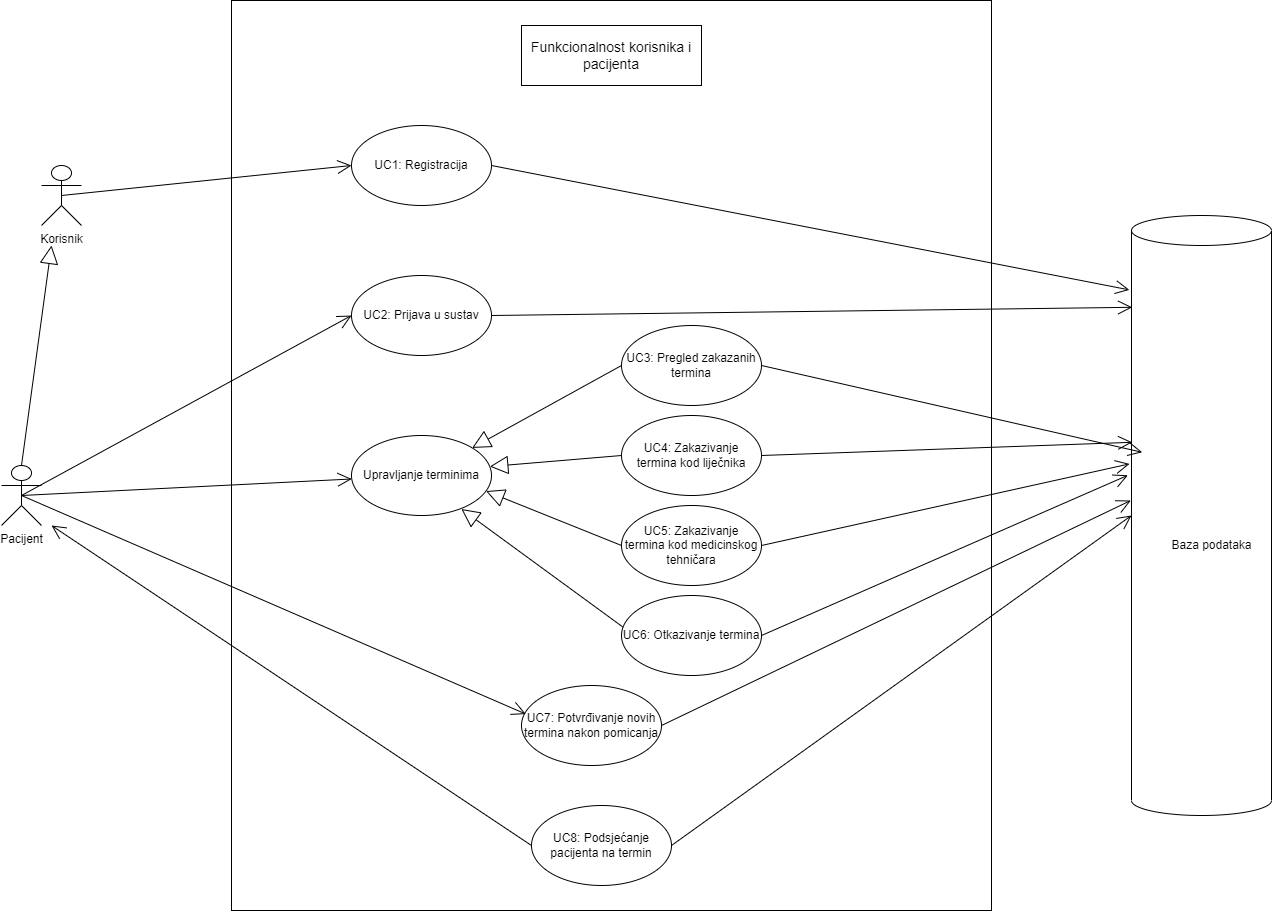
\includegraphics[width=\textwidth]{slike/pacijent_usecase_v2.png} %veličina u odnosu na širinu linije
			            \caption{Dijagram obrasca uporabe, funkcionalnost korisnika i pacijenta}
			            \label{fig:promjene2} %label mora biti drugaciji za svaku sliku
		            \end{figure}
				
				    \begin{figure}[H]
			            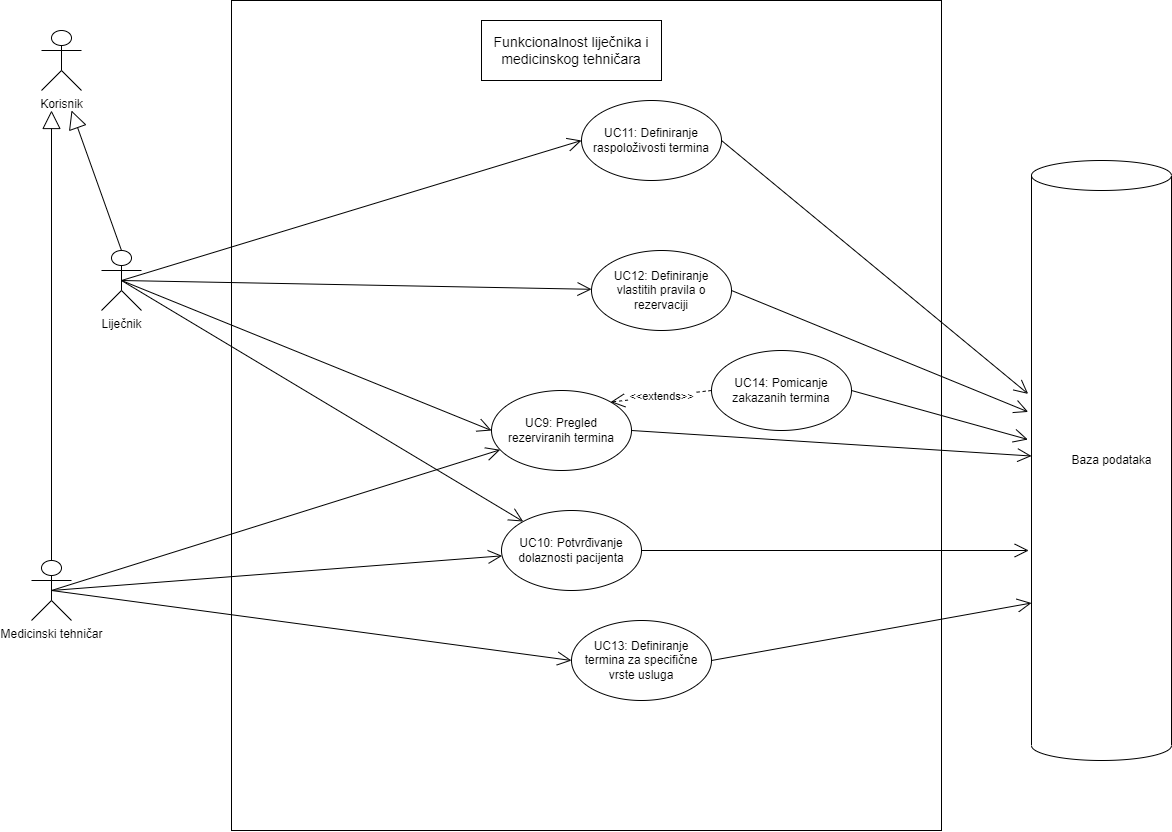
\includegraphics[width=\textwidth]{slike/lijecnik_tehn_usecase_v2.png} %veličina u odnosu na širinu linije
			            \caption{Dijagram obrasca uporabe, funkcionalnost liječnika i medicinskog tehničara/sestre}
			            \label{fig:promjene2} %label mora biti drugaciji za svaku sliku
		            \end{figure}
				
				    \begin{figure}[H]
			            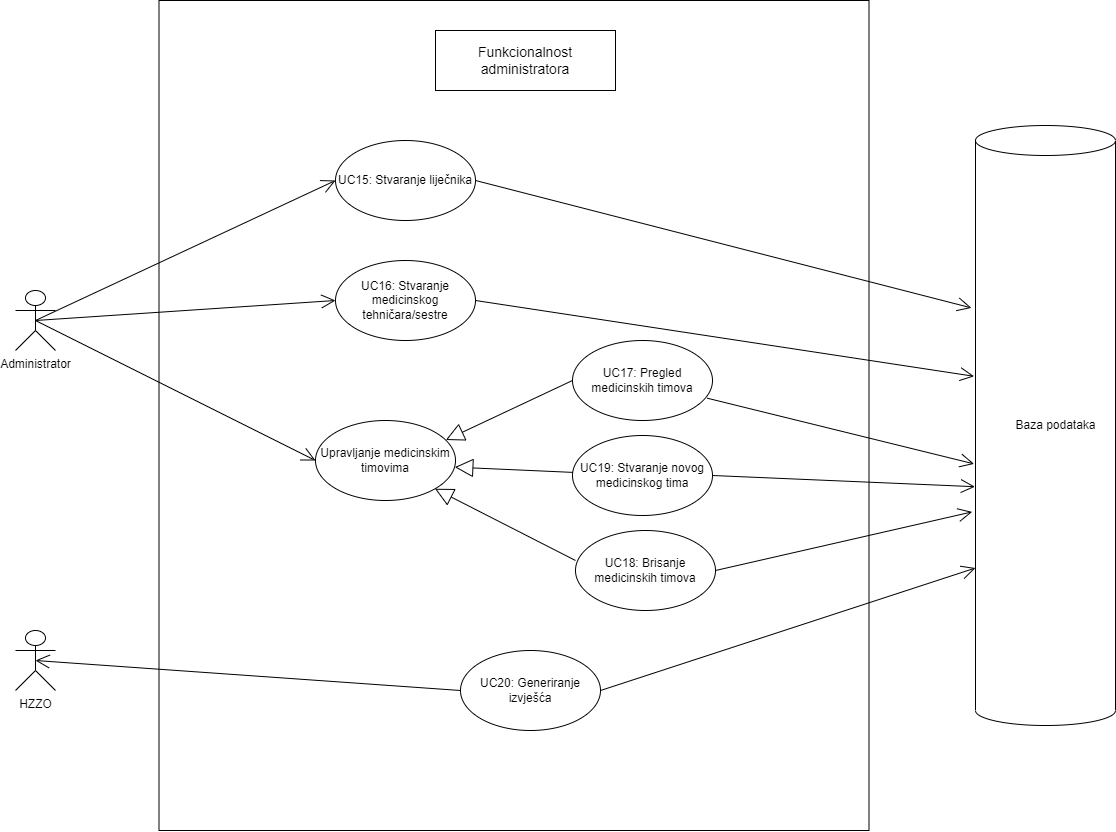
\includegraphics[width=\textwidth]{slike/administrator_usecase_v2.png} %veličina u odnosu na širinu linije
			            \caption{Dijagram obrasca uporabe, funkcionalnost administratora}
			            \label{fig:promjene2} %label mora biti drugaciji za svaku sliku
		            \end{figure}
		            
		            \eject
		            
			\subsection{Sekvencijski dijagrami}
				
				\subsubsection{Obrazac uporabe UC4 - Zakazivanje termina kod liječnika}
				Korisnik, prijavljen kao pacijent, želi vidjeti kalendar sa svojim terminima kako bi mogao zakazati sljedeći termin. Poslužitelj dohvaća trenutne termine i prikazuje ih. Korisnik želi zatražiti novi termin kod liječnika, međutim poslužitelj najprije mora provjeriti koji je status korisnika. Ako je sve u redu, pacijent je redovan, i poslužitelj dohvaća slobodne termine korisnikovog liječnika iz baze podataka i prikazuje ih korisniku. Korisnik bira željeni termin i dodatno naznačuje tip pregleda. Poslužitelj šalje nove podatke u bazu te obavještava korisnika te mu osvježava  kalendar. Ako je u korisnikovom statusu označeno da ima previše izostanaka sa zakazanih termina ili je zakazao previše termina, poslužitelj odbija zakazati novi termin i šalje odgovarajuću poruku korisniku.
				
				
				\begin{figure}[H]
			            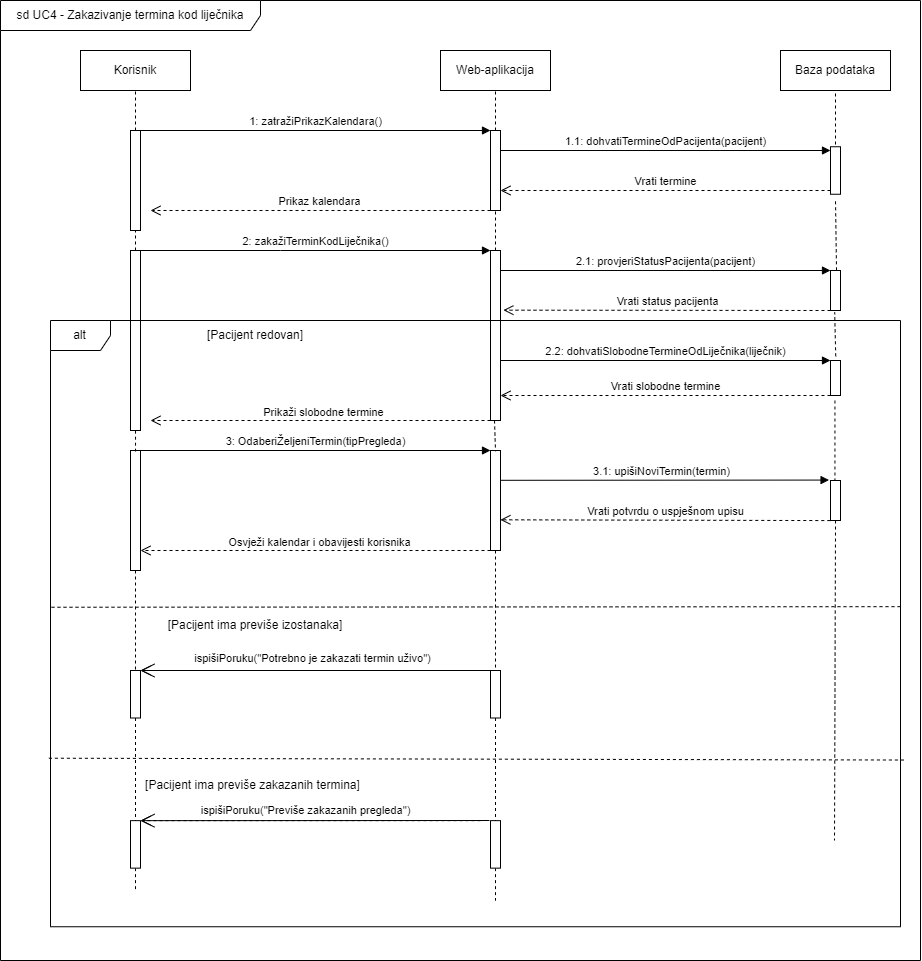
\includegraphics[width=\textwidth]{slike/sd_uc4_v2.png} %veličina u odnosu na širinu linije
			            \caption{Sekvencijski dijagram za UC4}
			            \label{fig:promjene2} %label mora biti drugaciji za svaku sliku
		            \end{figure}
		            
		        \eject
				
				\subsubsection{Obrazac uporabe UC6 - Otkazivanje termina}
				
				Korisnik, prijavljen kao pacijent, želi vidjeti kalendar sa svojim terminima kako bi mogao otkazati sljedeći termin. Poslužitelj dohvaća trenutne termine i prikazuje ih. Korisnik želi otkazati termin te na svom kalendaru pronalazi željeni termin i otkazuje ga. Poslužitelj tada najprije provjera koliko je vremena prošlo od rezervacije zadanog termina. Ako je prošlo više od 24 sata, tada poslužitelj odbija otkazati termin uz odgovarajuću poruku korisniku. Inače, poslužitelj šalje bazi podatak o terminu kojeg treba obrisati, te na potvrdu baze o uspješnom brisanju obavještava korisnika i osvježava mu kalendar.
				
				\begin{figure}[H]
			            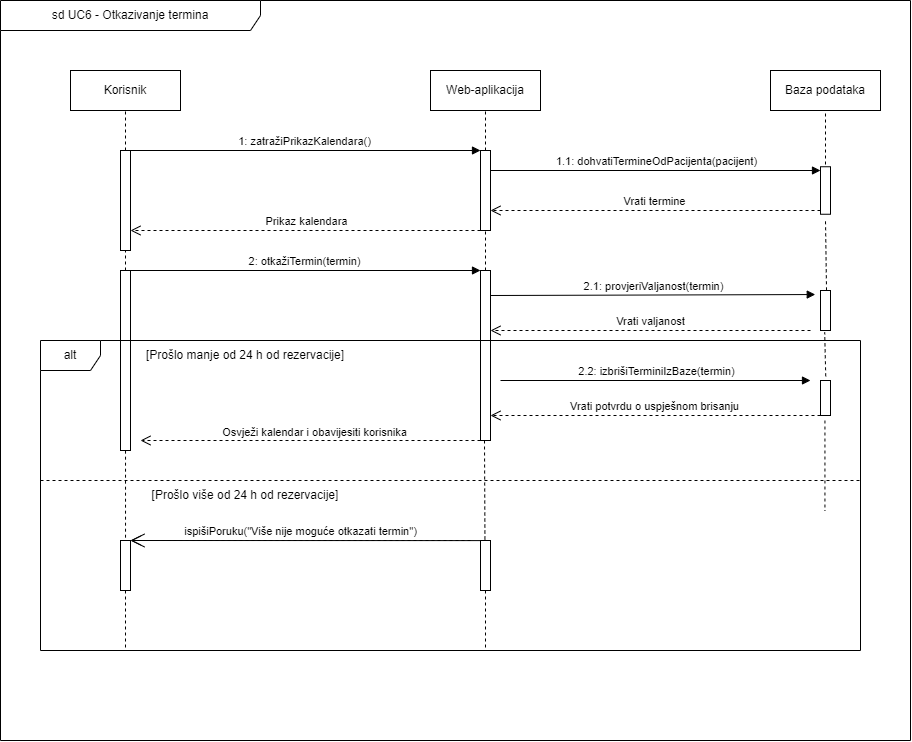
\includegraphics[width=\textwidth]{slike/sd_uc6.png} %veličina u odnosu na širinu linije
			            \caption{Sekvencijski dijagram za UC6}
			            \label{fig:promjene2} %label mora biti drugaciji za svaku sliku
		        \end{figure}
		            
		        \eject
		            
		            
				\subsubsection{Obrazac uporabe UC11 - Definiranje raspoloživosti termina}
				
				Korisnik, prijavljen kao liječnik, želi vidjeti kalendar kako bi imao uvid u svoje termine i mogao definirati njihovu raspoloživost. Poslužitelj dohvaća trenutne termine i prikazuje ih. Nakon što korisnik odluči definirati termine, poslužitelj mu vraća formu koja mu to omogućuje. Korisnik ima mogućnost definiranja termina sve dok ne potvrdi promjene. Nakon što korisnik potvrdi promjene, poslužitelj signalizira bazi da ih spremi. Poslije potvrde baze, poslužitelj osvježava korisnikov kalendar.
				
				\begin{figure}[H]
			            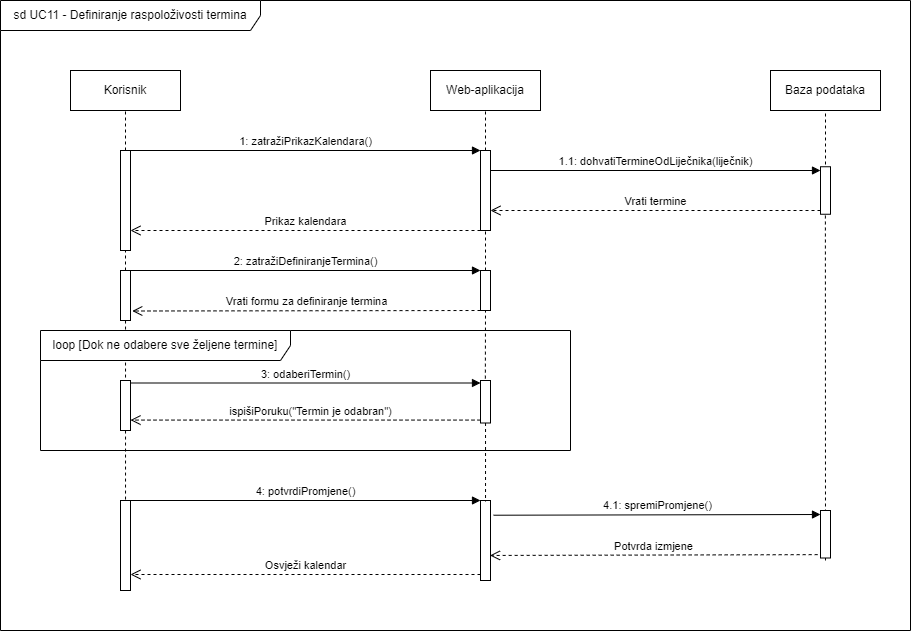
\includegraphics[width=\textwidth]{slike/sd_uc11.png} %veličina u odnosu na širinu linije
			            \caption{Sekvencijski dijagram za UC11}
			            \label{fig:promjene2} %label mora biti drugaciji za svaku sliku
		        \end{figure}
		        
		        \eject

		\section{Ostali zahtjevi}
			
			 \begin{packed_item}
			     \item Sustav treba biti izveden kao web aplikacija kojoj će korisnici pristupati uz pomoć korisničkog imena i lozinke
			     \item Oblikovanje aplikacije mora slijediti načela objektno-orijentiranog programiranja
			     \item Aplikacija treba biti jednostavna za korištenje, a sučelje pregledno i intuitivno
			     \item  Korisničko sučelje i sustav moraju podržavati hrvatsku abecedu (dijakritičke znakove) pri unosu i prikazu tekstualnog sadržaja
			     \item Sustav treba podržavati rad više korisnika u stvarnom vremenu
			     \item Neispravno korištenje korisničkog sučelja ne smije narušiti funkcionalnost i rad sustava
			     \item Veza s bazom podataka mora biti kvalitetno zastičena, brza i otporna na vanjske greške
			     \item Generirana dnevna i mjesečna izvješća o učinkovitosti šalju se u XML formatu
			     
			 \end{packed_item}
			 
			 
			 
	